% !TeX recipe = Tectonic
% CV - Marko Rosic - tailored for JetBrains, Senior Product Designer (AIR)
% Compile with: cd cv && tectonic Marko_Rosic_CV_jetbrains.tex
\documentclass[a4paper,9.5pt]{article}

% ── Font ──────────────────────────────────────────────────────────────
\usepackage{fontspec}
\setmainfont{Fira Sans}[
  BoldFont       = {Fira Sans Bold},
  ItalicFont     = {Fira Sans Italic},
  BoldItalicFont = {Fira Sans Bold Italic}
]
\newfontfamily\symfont{Zapf Dingbats}

% ── Layout ────────────────────────────────────────────────────────────
\usepackage[a4paper, top=1.5cm, bottom=1.4cm, left=1.8cm, right=1.8cm]{geometry}
\usepackage{microtype}

% ── Colors ────────────────────────────────────────────────────────────
\usepackage{xcolor}
\definecolor{darktext}{HTML}{111111}
\definecolor{midgray}{HTML}{555555}
\definecolor{lightgray}{HTML}{999999}
\definecolor{hairline}{HTML}{BBBBBB}

% ── Links ─────────────────────────────────────────────────────────────
\usepackage[hidelinks]{hyperref}
\urlstyle{same}
\usepackage[normalem]{ulem}

% ── Lists ─────────────────────────────────────────────────────────────
\usepackage{enumitem}

% ── Tables ────────────────────────────────────────────────────────────
\usepackage{array}

% ── TikZ ──────────────────────────────────────────────────────────────
\usepackage{tikz}
\usetikzlibrary{calc}

% ── Needspace ─────────────────────────────────────────────────────────
\usepackage{needspace}

% ── Section headings ──────────────────────────────────────────────────
\usepackage{titlesec}
\titleformat{\section}
  {\normalfont\small\bfseries}
  {}{0em}{\MakeUppercase}
  [\vspace{3pt}{\color{darktext}\hrule height 0.4pt}]
\titlespacing*{\section}{0pt}{22pt}{12pt}

% ── Page style ────────────────────────────────────────────────────────
\pagestyle{empty}
\setlength{\parindent}{0pt}
\setlength{\parskip}{0pt}

% ── Column dimensions ─────────────────────────────────────────────────
\newlength{\cvdatecol}  \setlength{\cvdatecol}{2.5cm}
\newlength{\cvsymcol}   \setlength{\cvsymcol}{1cm}
\newlength{\cvcontcol}  \setlength{\cvcontcol}{\dimexpr\textwidth-\cvdatecol-\cvsymcol\relax}

% ── Symbol counter ────────────────────────────────────────────────────
\newcounter{cvsymn}
\newif\ifcvfirst\cvfirsttrue

% ── TikZ asterisk with named remember-picture node ───────────────────
\newcommand{\cvastsym}{%
  \begin{tikzpicture}[remember picture, baseline=(sym-\thecvsymn.base)]
    \node[inner sep=0pt, outer sep=0pt, text=darktext, font=\normalsize\symfont] (sym-\thecvsymn) {✱};
  \end{tikzpicture}%
}

% ── Portfolio button ──────────────────────────────────────────────────
\newcommand{\portfoliobutton}{%
  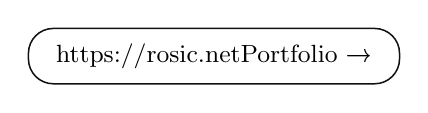
\begin{tikzpicture}[baseline=(btn.base)]
    \node[draw=darktext, rounded corners=9pt,
          inner xsep=10pt, inner ysep=5.5pt,
          line width=0.55pt, font=\small,
          outer sep=0pt] (btn)
      {\href{https://rosic.net}{Portfolio~→}};
  \end{tikzpicture}%
}

% ── Connector: hairline from prev asterisk to current, same page only ─
\newdimen\cvyprev
\newdimen\cvycurr
\newcommand{\cvdrawconnect}{%
  \edef\prevn{\the\numexpr\value{cvsymn}-1\relax}%
  \begin{tikzpicture}[overlay, remember picture]
    \coordinate (cvprev) at (sym-\prevn.center);
    \coordinate (cvcurr) at (sym-\thecvsymn.center);
    \pgfextracty{\cvyprev}{\pgfpointanchor{cvprev}{center}}%
    \pgfextracty{\cvycurr}{\pgfpointanchor{cvcurr}{center}}%
    \ifdim\cvyprev>\cvycurr%
      \draw[line width=0.35pt, color=hairline]
        ($(sym-\prevn)+(0,-4.5pt)$) -- ($(sym-\thecvsymn)+(0,4.5pt)$);%
    \fi%
  \end{tikzpicture}%
}

% ── Entry without company note ────────────────────────────────────────
\newcommand{\cventry}[3]{%
  \stepcounter{cvsymn}%
  \par\vspace{13pt}%
  \noindent%
  \makebox[\cvdatecol][r]{\small\bfseries\color{midgray}#1}%
  \makebox[\cvsymcol][c]{\cvastsym}%
  \parbox[t]{\cvcontcol}{%
    {\bfseries #2}\\[2.5pt]
    {\small#3}%
  }%
  \ifcvfirst\cvfirstfalse\else\cvdrawconnect\fi%
  \par%
}

% ── Entry with italic company context line ────────────────────────────
\newcommand{\cventrynote}[4]{%
  \stepcounter{cvsymn}%
  \par\vspace{13pt}%
  \noindent%
  \makebox[\cvdatecol][r]{\small\bfseries\color{midgray}#1}%
  \makebox[\cvsymcol][c]{\cvastsym}%
  \parbox[t]{\cvcontcol}{%
    {\bfseries #2}\\[2.5pt]
    {\small#3}\\[2.5pt]
    {\footnotesize\itshape\color{lightgray}#4}%
  }%
  \ifcvfirst\cvfirstfalse\else\cvdrawconnect\fi%
  \par%
}

% ── Bullet list ───────────────────────────────────────────────────────
\newenvironment{cvitems}{%
  \vspace{1pt}%
  \begin{itemize}[
    leftmargin = \dimexpr\cvdatecol+\cvsymcol+0.55em\relax,
    label      = {•},
    topsep     = 4pt,
    itemsep    = 3pt,
    parsep     = 0pt,
    partopsep  = 0pt
  ]\small\interlinepenalty=10000%
}{\end{itemize}}

% ── Skill block ───────────────────────────────────────────────────────
\newcommand{\skillblock}[2]{%
  {\small\bfseries #1}\newline%
  {\small\color{midgray}#2}%
}

% ══════════════════════════════════════════════════════════════════════
\begin{document}
% ══════════════════════════════════════════════════════════════════════

% ── HEADER ────────────────────────────────────────────────────────────
\vspace*{-0.3cm}
\noindent{\fontsize{30}{36}\selectfont\bfseries Marko Rosić}%
\hfill\makebox[0pt][r]{\portfoliobutton\hspace{2pt}}
\par\vspace{3pt}
{\small\color{midgray}%
  Cara Du\v{s}ana 118, Belgrade, Serbia~\textbar~%
  +381 60 585 44 55~\textbar~%
  \href{mailto:marko@rosic.net}{\uline{marko@rosic.net}}~\textbar~%
  \href{https://rosic.net}{\uline{rosic.net}}%
}

% ── SUMMARY ───────────────────────────────────────────────────────────
\section{Summary}

{\small Product designer with 15+ years building complex, functional products
at the intersection of design and engineering. I design systems that hold up
as things grow (−30\% dev time, −25\% time-to-market) and work closely with
engineering to make sure design translates correctly into code. I have
experience designing complex backend tooling and functional technical
interfaces, and I use Claude Code and AI agents daily to build and prototype.
Designing for a product I already rely on as part of my workflow brings
direct user insight to the work.}

% ── EXPERIENCE ────────────────────────────────────────────────────────
\section{Experience}

\cventry{5/2025\,--\,Present}{Design Leadership Consultant}{%
  Beyond Clicks Studio (Independent) \textbar{} Belgrade, Serbia (Remote)}
\begin{cvitems}
  \item Senior design lead across concurrent client engagements covering
        design systems, product strategy, and design-engineering workflow
  \item Led AI-orchestrated product delivery using Claude Code: owned
        problem definition, UX, and research while using AI agents to build
        faster; shipped a working internal operations product end to end
  \item Designed and built Figma plugins that close the gap between what
        is designed and what gets built
  \item Directed multi-brand design-system work for an international media
        group: token architecture, component conventions, and engineering
        handoff
\end{cvitems}

\cventrynote{7/2024\,--\,5/2025}{Head of UX/UI}{%
  Gentoo Media \textbar{} Belgrade, Serbia}{%
  Gentoo Media was established following GiG Media's acquisition of
  Catena Media and subsequent spin-off of its media division.}
\begin{cvitems}
  \item Built a company-wide design system across multi-brand products,
        setting the standard for product design across the organisation
  \item Led a design team of seven and cut time-to-market for new
        features by 25\%
  \item Worked closely with engineering so design fit how they built
\end{cvitems}

\cventry{5/2021\,--\,7/2024}{Lead UX/UI Designer}{%
  Catena Media (acquired by GiG Media in 2023) \textbar{} Belgrade, Serbia}
\begin{cvitems}
  \item Built a design system for the flagship consumer product that cut
        development time by 30\%, then scaled it across 10+ websites
  \item Directed UX end to end for high-traffic, multi-market consumer
        web products using user-centred methods
  \item Mentored junior designers and built a team that worked well
        independently
  \item Ran workshops with stakeholders to line up design decisions with
        business goals
\end{cvitems}

\cventry{10/2018\,--\,5/2021}{Senior UX/UI Designer}{%
  Catena Media \textbar{} Belgrade, Serbia}
\begin{cvitems}
  \item Led the redesign of the flagship consumer product, raising mobile
        traffic by 20\% and user retention by 15\%
  \item Brought UX research into the product process and moved the team
        to evidence-based decisions
  \item Moved the team from Sketch to Figma, improving how designers and
        engineers worked together
\end{cvitems}

\needspace{5\baselineskip}
\cventry{12/2013\,--\,10/2018}{Interaction Designer}{%
  Smith Micro Software, Inc \textbar{} Belgrade, Serbia}
\begin{cvitems}
  \item Designed UX for carrier-branded Android apps shipped with Sprint
        and T-Mobile, including Visual Voicemail and messaging apps.
        Complex functional interfaces built to strict carrier and platform
        specifications
  \item Designed backend tooling for device management and an IoT
        location-based notification system, working at the intersection of
        consumer-facing UX and complex operational interfaces
  \item Won Best of Swiss Apps Gold (Entertainment) for Swisscom TV
        Android tablet app (2013)
\end{cvitems}

\cventry{2009\,--\,2013}{UI Designer}{%
  MySkin, Youngculture \textbar{} Belgrade, Serbia}
\begin{cvitems}
  \item Designed digital products and interfaces across client projects
\end{cvitems}

\cventry{2005\,--\,2008}{Co-founder \& CEO}{%
  Mainstream d.o.o. \textbar{} Belgrade, Serbia}
\begin{cvitems}
  \item Co-founded a dial-up ISP; led operations and product design
        during the founding phase
\end{cvitems}

\cventry{2000\,--\,2005}{Web Designer/Developer}{%
  Various companies \textbar{} Belgrade, Serbia}

% ── SKILLS ────────────────────────────────────────────────────────────
\section{Skills}

\vspace{2pt}
\noindent
\begin{minipage}[t]{0.475\textwidth}
  \skillblock{Design \& Research}{%
    Figma, Axure RP, HTML/JS prototyping,
    Design Systems, Component Libraries,
    Interaction Design, Visual Design,
    User Research \& Usability Testing
    (UserZoom, Optimal Workshop, HotJar)}

  \vspace{12pt}
  \skillblock{Data \& Analytics}{%
    Google Analytics, VWO, HotJar,
    Usability Testing, A/B Testing}
\end{minipage}%
\hspace{0.05\textwidth}%
\begin{minipage}[t]{0.475\textwidth}
  \skillblock{Technical}{%
    HTML/CSS, JavaScript,
    Figma Plugin Development,
    AI-orchestrated delivery (Claude Code),
    MVP/POC Prototyping,
    Dev Complexity Assessment}

  \vspace{12pt}
  \skillblock{Leadership \& Ops}{%
    Design Ops, Team Leadership \& Mentoring,
    Cross-functional Stakeholder Management,
    Roadmap Planning,
    Jira, Asana, Linear, Notion}
\end{minipage}

% ── LANGUAGES ─────────────────────────────────────────────────────────
\section{Languages}

\begin{itemize}[leftmargin=1.2em, label={•},
    topsep=0pt, itemsep=2pt, parsep=0pt]
  \item {\small\textbf{English:} Fluent (Business Proficiency)}
  \item {\small\textbf{French:} Intermediate}
\end{itemize}

% ── EDUCATION ─────────────────────────────────────────────────────────
\section{Education}

\noindent{\small\bfseries Bachelor of Economics}\\[1pt]
{\small\color{midgray}Faculty for Business Studies,
Megatrend University, Belgrade \hfill 2002\,--\,2008}

\vspace{6pt}

\noindent{\small\bfseries Industrial Design Technician}\\[1pt]
{\small\color{midgray}School for Design, Belgrade
\hfill 1995\,--\,1999}

% ── CERTIFICATIONS ────────────────────────────────────────────────────
\section{Certifications}

\noindent{\small\bfseries User Research --- Methods and Best Practices}\\[1pt]
{\small\color{midgray}Interaction Design Foundation
\hfill 2017}

% ── AWARDS ────────────────────────────────────────────────────────────
\section{Awards}

\noindent{\small Best of Swiss Apps --- Gold (Entertainment), Swisscom TV
Android tablet app. 2013.}

\end{document}
